\documentclass[14pt]{extbook}
\usepackage{multicol, enumerate, enumitem, hyperref, color, soul, setspace, parskip, fancyhdr} %General Packages
\usepackage{amssymb, amsthm, amsmath, bbm, latexsym, units, mathtools} %Math Packages
\everymath{\displaystyle} %All math in Display Style
% Packages with additional options
\usepackage[headsep=0.5cm,headheight=12pt, left=1 in,right= 1 in,top= 1 in,bottom= 1 in]{geometry}
\usepackage[usenames,dvipsnames]{xcolor}
\usepackage{dashrule}  % Package to use the command below to create lines between items
\newcommand{\litem}[1]{\item#1\hspace*{-1cm}\rule{\textwidth}{0.4pt}}
\pagestyle{fancy}
\lhead{Progress Quiz 5}
\chead{}
\rhead{Version B}
\lfoot{9912-2038}
\cfoot{}
\rfoot{Spring 2021}
\begin{document}

\begin{enumerate}
\litem{
Determine the domain of the function below.\[ f(x) = \frac{4}{18x^{2} -45 x + 25} \]\begin{enumerate}[label=\Alph*.]
\item \( \text{All Real numbers except } x = a, \text{ where } a \in [14.3, 15.5] \)
\item \( \text{All Real numbers except } x = a \text{ and } x = b, \text{ where } a \in [0.2, 1.5] \text{ and } b \in [1.6, 2.1] \)
\item \( \text{All Real numbers.} \)
\item \( \text{All Real numbers except } x = a \text{ and } x = b, \text{ where } a \in [14.3, 15.5] \text{ and } b \in [29.2, 32.1] \)
\item \( \text{All Real numbers except } x = a, \text{ where } a \in [0.2, 1.5] \)

\end{enumerate} }
\litem{
Choose the graph of the equation below.\[ f(x) = \frac{-1}{(x - 3)^2} + 1 \]\begin{enumerate}[label=\Alph*.]
\begin{multicols}{2}\item 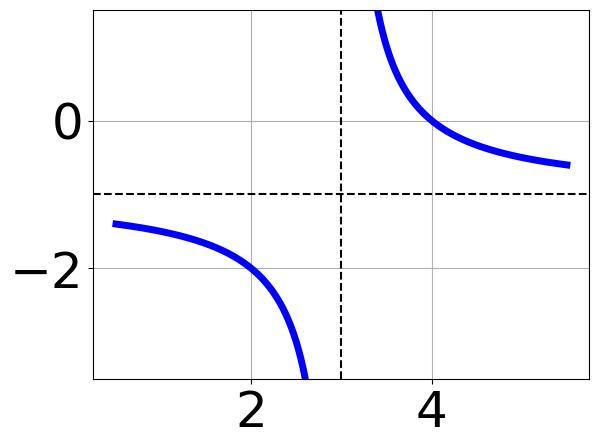
\includegraphics[width = 0.3\textwidth]{../Figures/rationalEquationToGraphCopyAB.png}\item 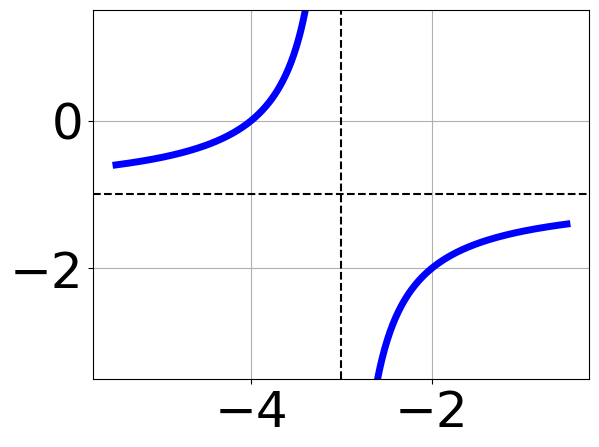
\includegraphics[width = 0.3\textwidth]{../Figures/rationalEquationToGraphCopyBB.png}\item 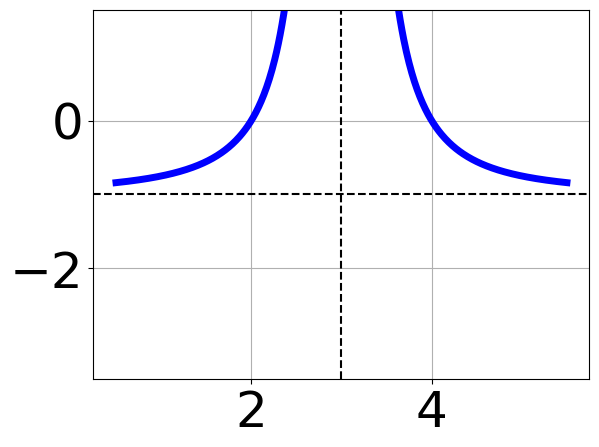
\includegraphics[width = 0.3\textwidth]{../Figures/rationalEquationToGraphCopyCB.png}\item 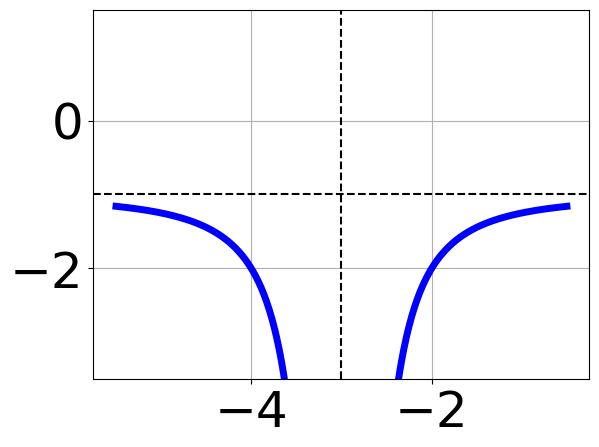
\includegraphics[width = 0.3\textwidth]{../Figures/rationalEquationToGraphCopyDB.png}\end{multicols}\item None of the above.
\end{enumerate} }
\litem{
Choose the equation of the function graphed below.
\begin{center}
    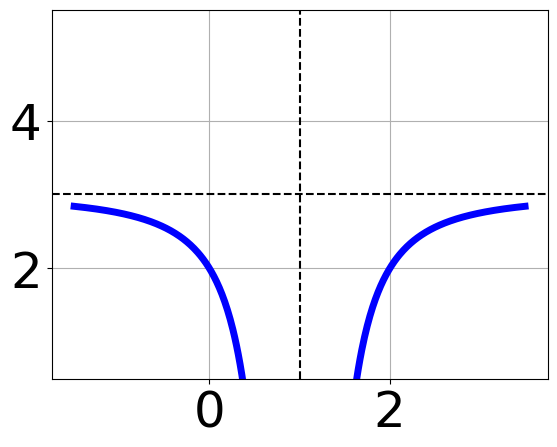
\includegraphics[width=0.5\textwidth]{../Figures/rationalGraphToEquationCopyB.png}
\end{center}
\begin{enumerate}[label=\Alph*.]
\item \( f(x) = \frac{1}{(x + 1)^2} + 3 \)
\item \( f(x) = \frac{-1}{x - 1} + 3 \)
\item \( f(x) = \frac{-1}{(x - 1)^2} + 3 \)
\item \( f(x) = \frac{1}{x + 1} + 3 \)
\item \( \text{None of the above} \)

\end{enumerate} }
\litem{
Choose the graph of the equation below.\[ f(x) = \frac{1}{x + 3} + 3 \]\begin{enumerate}[label=\Alph*.]
\begin{multicols}{2}\item 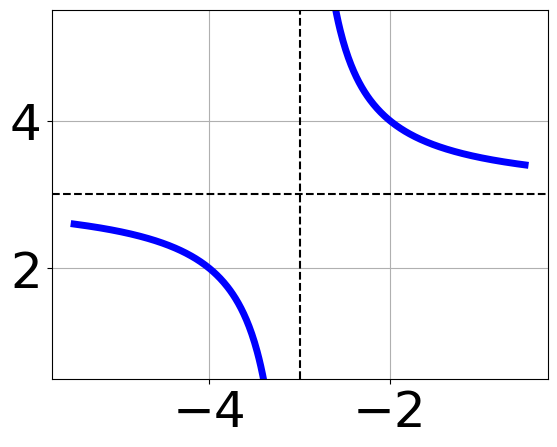
\includegraphics[width = 0.3\textwidth]{../Figures/rationalEquationToGraphAB.png}\item 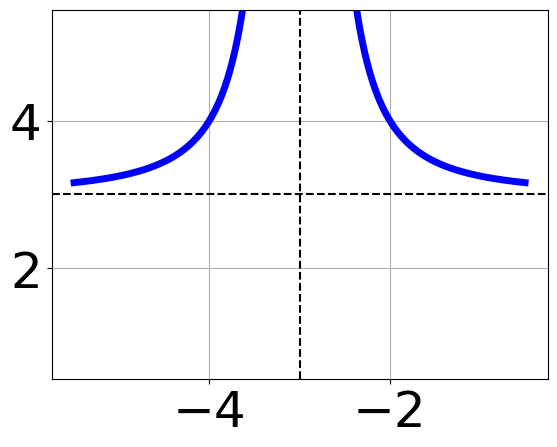
\includegraphics[width = 0.3\textwidth]{../Figures/rationalEquationToGraphBB.png}\item 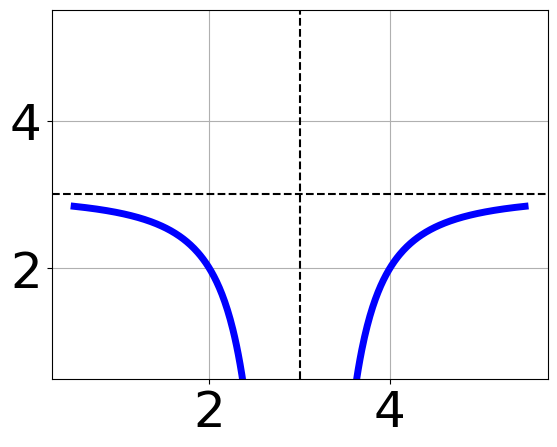
\includegraphics[width = 0.3\textwidth]{../Figures/rationalEquationToGraphCB.png}\item 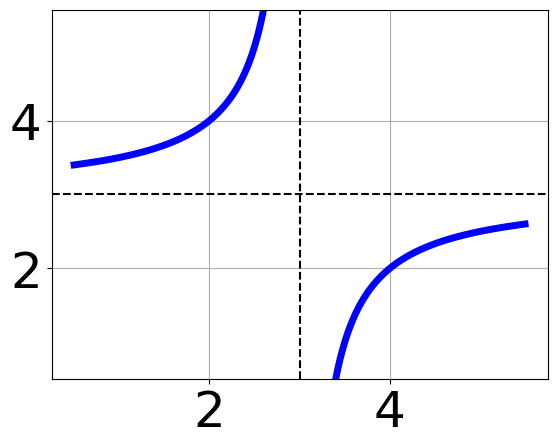
\includegraphics[width = 0.3\textwidth]{../Figures/rationalEquationToGraphDB.png}\end{multicols}\item None of the above.
\end{enumerate} }
\litem{
Solve the rational equation below. Then, choose the interval(s) that the solution(s) belongs to.\[ \frac{78}{-52x -78} + 1 = \frac{78}{-52x -78} \]\begin{enumerate}[label=\Alph*.]
\item \( \text{All solutions lead to invalid or complex values in the equation.} \)
\item \( x \in [-1.5,-0.5] \)
\item \( x_1 \in [-1.5, -0.5] \text{ and } x_2 \in [-2.5,0.5] \)
\item \( x \in [0.5,3.5] \)
\item \( x_1 \in [-1.5, -0.5] \text{ and } x_2 \in [1.5,4.5] \)

\end{enumerate} }
\litem{
Solve the rational equation below. Then, choose the interval(s) that the solution(s) belongs to.\[ \frac{7x}{-2x -2} + \frac{-6x^{2}}{6x^{2} -8 x -14} = \frac{2}{-3x + 7} \]\begin{enumerate}[label=\Alph*.]
\item \( x_1 \in [-0.22, 0.42] \text{ and } x_2 \in [0.04,4.04] \)
\item \( x \in [1.73,2.25] \)
\item \( x_1 \in [-0.22, 0.42] \text{ and } x_2 \in [-3,1] \)
\item \( x \in [2.31,2.61] \)
\item \( \text{All solutions lead to invalid or complex values in the equation.} \)

\end{enumerate} }
\litem{
Determine the domain of the function below.\[ f(x) = \frac{6}{9x^{2} +9 x -18} \]\begin{enumerate}[label=\Alph*.]
\item \( \text{All Real numbers except } x = a, \text{ where } a \in [-20, -17] \)
\item \( \text{All Real numbers except } x = a \text{ and } x = b, \text{ where } a \in [-3, -1] \text{ and } b \in [1, 2] \)
\item \( \text{All Real numbers except } x = a \text{ and } x = b, \text{ where } a \in [-20, -17] \text{ and } b \in [6, 11] \)
\item \( \text{All Real numbers except } x = a, \text{ where } a \in [-3, -1] \)
\item \( \text{All Real numbers.} \)

\end{enumerate} }
\litem{
Solve the rational equation below. Then, choose the interval(s) that the solution(s) belongs to.\[ \frac{90}{-50x -40} + 1 = \frac{90}{-50x -40} \]\begin{enumerate}[label=\Alph*.]
\item \( x_1 \in [-1.4, 0.5] \text{ and } x_2 \in [0,1.1] \)
\item \( \text{All solutions lead to invalid or complex values in the equation.} \)
\item \( x \in [0.1,1.4] \)
\item \( x_1 \in [-1.4, 0.5] \text{ and } x_2 \in [-0.9,-0.1] \)
\item \( x \in [-1.8,0.2] \)

\end{enumerate} }
\litem{
Solve the rational equation below. Then, choose the interval(s) that the solution(s) belongs to.\[ \frac{-6x}{6x + 6} + \frac{-2x^{2}}{-18x^{2} +24 x + 42} = \frac{6}{-3x + 7} \]\begin{enumerate}[label=\Alph*.]
\item \( \text{All solutions lead to invalid or complex values in the equation.} \)
\item \( x \in [1.71,2.96] \)
\item \( x \in [4.08,6.5] \)
\item \( x_1 \in [-1.61, 0.2] \text{ and } x_2 \in [5.3,11.3] \)
\item \( x_1 \in [-1.61, 0.2] \text{ and } x_2 \in [-3,5] \)

\end{enumerate} }
\litem{
Choose the equation of the function graphed below.
\begin{center}
    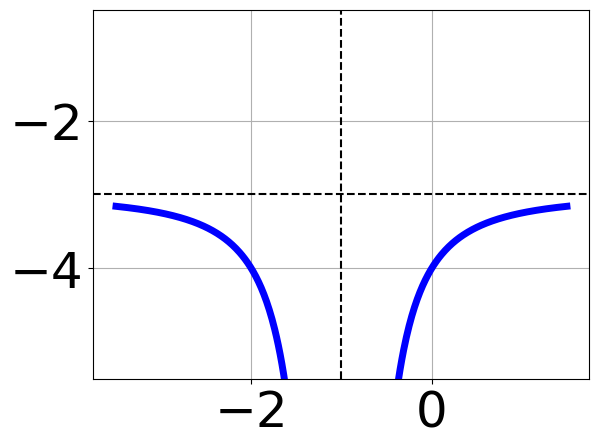
\includegraphics[width=0.5\textwidth]{../Figures/rationalGraphToEquationB.png}
\end{center}
\begin{enumerate}[label=\Alph*.]
\item \( f(x) = \frac{1}{(x - 1)^2} - 3 \)
\item \( f(x) = \frac{-1}{x + 1} - 3 \)
\item \( f(x) = \frac{1}{x - 1} - 3 \)
\item \( f(x) = \frac{-1}{(x + 1)^2} - 3 \)
\item \( \text{None of the above} \)

\end{enumerate} }
\end{enumerate}

\end{document}